\section{Results}
\label{sec:results}

\subsection{The design did not meet its capacity requirements}
After the 96 primary files and all four alternate rounds had been processed, the evaluation set contained 150 unique station--observation opportunities. This was 37.5\% of the required total of 400. The smallest station--block count was zero, and only three of the 40 cells reached the requirement of eight. Both parts of the capacity rule therefore failed. The source workflow recorded \texttt{G0\_NOT\_PASSED} and \texttt{FAIL\_EXHAUSTED}, leaving the outcome-reading stage B1 unauthorized. These decisions concern support for the planned benchmark; the percentage does not measure archive completeness or wind-retrieval performance.

Table~\ref{tab:gate-results} distinguishes this capacity decision, \texttt{G0-v4.1}, from the subsequent replay-integrity decision, \texttt{G0-v5}. The replay passed because it reproduced the unsuccessful capacity check and its supporting records. It did not add observations or authorize the original performance experiment.

\begin{table*}[t]
\caption{Capacity and replay decisions. A successful replay does not change the capacity result.}
\label{tab:gate-results}
\centering
\small
\begin{tabularx}{\textwidth}{@{}p{0.14\textwidth}p{0.23\textwidth}p{0.24\textwidth}X@{}}
\toprule
Decision & Observed result & Requirement & Consequence \\
\midrule
Capacity: \texttt{G0-v4.1} &
150 opportunities; minimum cell count 0; 3 of 40 cells reach 8 &
At least 400 overall and at least 8 in every station--block cell &
Failed after all alternate rounds; B1 remained closed. \\
Replay: \texttt{G0-v5} &
62 of 62 comparisons agree; 13 of 13 integrity checks pass &
Agreement with the sealed inputs, counts, decisions, and outcome-access record &
The capacity failure was reproduced; no performance evaluation was authorized. \\
\bottomrule
\end{tabularx}
\end{table*}

Figure~\ref{fig:capacity} shows the complete matrix, including zero-count cells. Station totals ranged from zero at 42056 to 35 at 44020; station 41047 contributed one opportunity. The remaining totals were 22 at 42001, 29 at 42035, 14 at 42036, 30 at 44008, and 19 at 44014. The three qualifying cells were 42035 in Block~4 and 44008 in Block~1, each with eight opportunities, and 44020 in Block~4, with nine. Thus, the shortfall was not confined to the overall total: most of the intended station--time comparisons also lacked the required support.


\begin{figure}[!t]
\centering
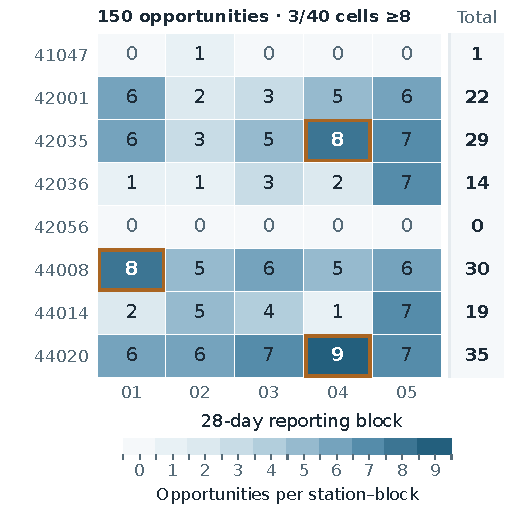
\includegraphics[width=\columnwidth]{figures/figure2.pdf}
\caption{Unique station--observation opportunities in the eight-station, five-block design. All cells, including zeros, are shown. Outlined cells reach the required eight opportunities; three of 40 do so.}
\label{fig:capacity}
\end{figure}

\subsection{Terminal states and the distribution of the shortfall}
Every one of the 1,536 station--file combinations received a final processing state. Of the 1,024 evaluation rows, 150 were valid extracts, 35 failed the two-candidate requirement, 628 had no spatial overlap, and 211 had an invalid time. The corresponding development counts were 68, 30, 271, and 143, totaling 512. Across both roles, the four counts were 218, 65, 899, and 354. Table~\ref{tab:accounting} summarizes these totals and the principal integrity checks; Fig.~\ref{fig:terminals} displays the role-specific composition.

The stored labels are \texttt{extract\_valid}, \texttt{fewer\_than\_two\_valid\_candidates}, \texttt{no\_overlap}, and \texttt{time\_invalid}. They identify the condition at which processing ended. A valid extract satisfies the predictor protocol but is not a claim of accurate wind retrieval; similarly, a failed extract does not by itself identify a physical cause.

\begin{table*}[t]
\caption{Terminal-state counts and principal record checks. Terminal counts use station--file rows, whereas the case manifest uses unique station--observation opportunities.}
\label{tab:accounting}
\centering
\small
\begin{minipage}[t]{0.48\textwidth}
\vspace{0pt}
\begin{tabularx}{\linewidth}{@{}Xrr@{}}
\toprule
Terminal state & Evaluation & Development \\
\midrule
Valid extract & 150 & 68 \\
Fewer than two valid candidates & 35 & 30 \\
No spatial overlap & 628 & 271 \\
Invalid time & 211 & 143 \\
\midrule
Total & 1,024 & 512 \\
\bottomrule
\end{tabularx}
\end{minipage}
\hfill
\begin{minipage}[t]{0.49\textwidth}
\vspace{0pt}
\begin{tabularx}{\linewidth}{@{}Xr@{}}
\toprule
Record check & Reported value \\
\midrule
Unique final keys & 1,942 \\
Retained nonfinal attempts & 253 \\
Parquet rows $\times$ ordered fields & $150\times22$ \\
Downloaded / reused source files & 125 / 3 \\
Transient raw files at closure & 0 \\
Recorded NDBC outcome reads & 0 \\
\bottomrule
\end{tabularx}
\end{minipage}
\end{table*}


\begin{figure}[!t]
\centering
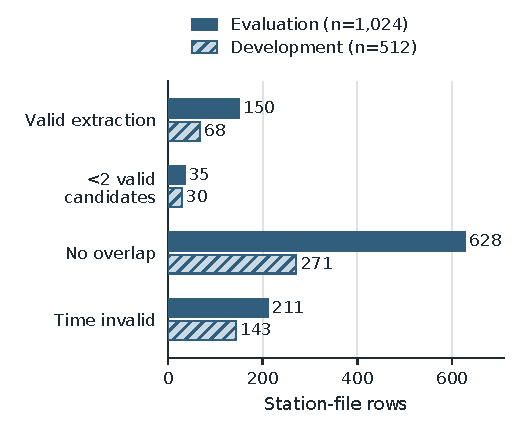
\includegraphics[width=\columnwidth]{figures/figure3.pdf}
\caption{Processing-state counts by station role. Evaluation and development denominators are 1,024 and 512 station--file records, respectively. The bars show counts, not rates; the state labels do not identify physical causes.}
\label{fig:terminals}
\end{figure}

\subsection{Opportunity gains along the prescribed acquisition sequence}
The primary set yielded 114 opportunities from 96 files and used 7,003,624,776 new science bytes. Successive complete alternate rounds added 11, 9, 11, and five opportunities, taking the cumulative totals to 125, 134, 145, and 150. Figure~\ref{fig:budget} plots the five realized stages. The additional byte costs were 610,514,454; 596,205,693; 590,329,239; and 617,772,188, respectively. Round~4 therefore had the lowest observed marginal opportunity yield. Exact cumulative values are retained in the supplementary inventory.

The complete sequence used 9,418,446,350 new science bytes, or 9.418 decimal GB. This left 581,553,650 bytes below the 10,000,000,000-byte limit, but no further alternate round was permitted. The final stop followed exhaustion of the registered file sequence, not depletion of every remaining byte. The five plotted points describe that sequence only; they do not establish an optimal file-selection policy or a budget frontier.


\begin{figure}[!t]
\centering
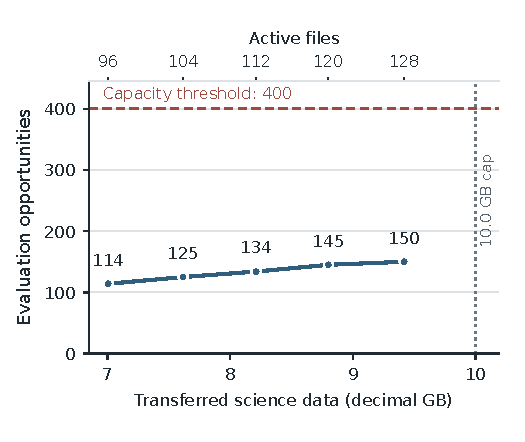
\includegraphics[width=\columnwidth]{figures/figure4.pdf}
\caption{Cumulative evaluation opportunities and acquisition cost after the primary set and each complete alternate round. Cost is in decimal GB and includes probe bytes. The points describe the executed sequence; the dashed line is the required total of 400 opportunities.}
\label{fig:budget}
\end{figure}

\subsection{Diagnostics by file stratum, station, and time block}
The further decompositions in Fig.~\ref{fig:diagnostics} use all 1,024 evaluation rows. No overlap was the largest category in each sector--platform--pass stratum, ranging from 72 of 128 rows (56.25\%) in both Atlantic MetOp-B strata to 84 of 128 (65.63\%) in the Atlantic MetOp-C descending and Gulf MetOp-B ascending strata. Atlantic-sector files contributed 89 valid opportunities and Gulf-sector files contributed 61.

The station breakdown was more uneven. All 128 rows at 42056 ended in no overlap, as did 112 of 128 at 41047. Invalid times were most frequent at 42036, with 50 of 128 rows. All rows in the block breakdown were grouped by source-file sensing time, because failed records lack a valid center-pixel block. Its denominators were consequently 184, 224, 176, 224, and 216, rather than equal-sized groups. These displays locate the recorded losses within the selected design; they do not separate station geography, orbit geometry, retrieval behavior, or archive state as explanations.


\begin{figure*}[!t]
\centering
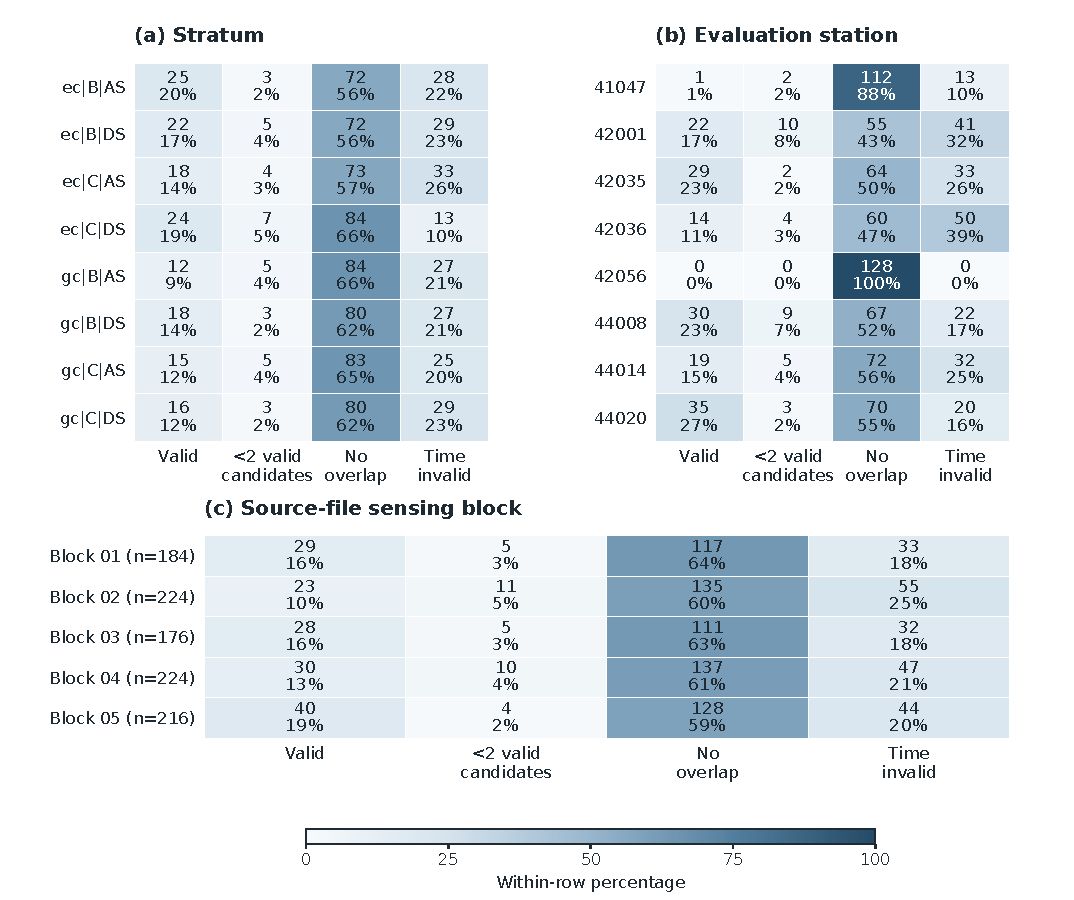
\includegraphics[width=\textwidth]{figures/figure5.pdf}
\caption{Evaluation processing states by (a) sector--platform--pass stratum, (b) station, and (c) source-file sensing block. In (a), ec/gc denote the Atlantic/Gulf product sectors, B/C denote MetOp-B/MetOp-C, and AS/DS denote ascending/descending passes. Cells show counts and within-row percentages. Each row in (a) and (b) has 128 records; the block denominators in (c) differ. All records in panel (c) are grouped by file sensing time, because failed records lack a valid center-pixel time. These are descriptive processing categories, not causal diagnoses.}
\label{fig:diagnostics}
\end{figure*}

\subsection{Closure, transfer accounting, and replay agreement}
The final record contained 128 selected-source keys, 128 source-transfer keys, 1,536 station-extract keys, and 150 predictor-case keys: 1,942 in total. No expected final key was missing or duplicated. A further 253 nonfinal attempts remained in the lineage with valid parent chains.

Of the 128 source files, 125 were newly downloaded and three reused existing geometry evidence with matching digests. Downloaded objects accounted for 9,418,445,350 bytes. The transaction added 1,000 probe bytes, consistent with 125 eight-byte probes, to obtain the total acquisition cost above. All newly downloaded raw files were deleted after their extracts had been verified; the three reused geometry files were retained.

The evaluation Parquet contained 150 rows and 22 ordered fields. It had 150 unique case identifiers and 150 unique station--observation keys. The file digest, schema digest, \texttt{PAR1} signature, dimensions, uniqueness checks, and reopen check agreed with the recorded contract. No prohibited outcome field was present.

The replay produced 62 ledger comparisons, all with matching observed and expected values, and passed all 13 registered integrity checks. The NDBC outcome-read counter remained zero, and no outcome path or field was found among the replay inputs. Accordingly, no wind error, calibration measure, ambiguity-comparison score, or model ranking was produced.

\subsection{Provenance limitations reproduced by the audit}
\label{sec:provenance}
Two weaknesses in the source record remained despite the successful checks. First, a nested Parquet receipt points to a temporary staging location that was deleted after commit. The canonical file passes the content, schema, uniqueness, and reopening checks, but the embedded locator is no longer usable. Content integrity and locator validity are therefore different properties in this record.

Second, the transfer lineage contains 125 \texttt{probe\_ok} nodes but does not retain an individual request-and-response receipt for each successful probe. The aggregate calculation, $125\times8=1{,}000$ bytes, reconciles; it cannot independently reconstruct every response header or returned magic byte. A later release could add a locator-resolution map without changing the original receipt and retain complete per-probe receipts for new acquisitions. Neither repair has been counted here as a completed experiment.

